\chapter{Resultaten met het ingebouwd model}
\label{ch:resultaten-ingebouwd-model}

De 845 beelden van Huis van Alijn werden getagd door het general model van Clarifai. Aan iedere foto werden twintig tags gegeven. De waarschijnlijkheidsscore van de tags bevond zich tussen 100\% en 65\% en had een gemiddelde van 93\%. 

De verkregen tags zijn op te delen in een aantal categorieën en gaan over verschillende aspecten van het beeld:
\begin{itemize}
	\item entiteiten die op de beelden te zien zijn, waaronder \textit{volwassene}, \textit{speelgoed}, \textit{bloem}, \textit{kameel}, \textit{jurk}, \textit{meubelen} en \textit{strand};
	\item activiteiten die uitgevoerd worden op de beelden, zoals \textit{dansen}, \textit{zitten}, \textit{rusten}, \textit{winkelen} en \textit{reizen};
	\item emoties of gevoelens die te zien zijn op het beeld of die opgeroepen worden door het beeld, denk aan \textit{plezier}, \textit{liefde}, \textit{genot}, \textit{avontuur}, \textit{affectie}, \textit{sexy} en \textit{mooi};
	\item maar ook contextuele concepten, zoals \textit{vriendschap}, \textit{familie}, \textit{toerisme}, \textit{vrije tijd} en \textit{het samen zijn};
	\item en hoeveelheden: \textit{één}, \textit{twee}, \textit{drie}, \textit{vier}, \textit{veel}, \textit{enkele}. Dit waren vaak weinigzeggende termen die opvallend vaak fout waren. Het was ook niet altijd duidelijk waar die hoeveelheden op sloegen. Veel mensen? Veel bloemen?
	\item tot slot kregen we ook informatie over de foto zelf: \textit{portret}, \textit{kleur}, \textit{zwart-wit}, \textit{sepia}, \textit{monochroom}...
\end{itemize}

Tijdens de validatie werd vastgesteld dat Clarifai veel algemene termen geeft, zoals \textit{mensen}, \textit{volwassene}, \textit{kind}, \textit{groep} en \textit{veel}, maar soms waren we ook verwonderd over de relevantie van de tags. Enkele van die relevante tags zijn: \textit{schildersezel}, \textit{roos}, \textit{uitstapje}, \textit{airbus}, \textit{souvenir}, \textit{bazaar}, \textit{grasland}, \textit{broche} en \textit{bruidsmeisje}. 

Na validatie bleken 11.517 van de 16.900 tags correct te zijn (68,15\%). Dit resulteerde in 371 unieke termen die de foto’s beschreven. Bij 21 foto’s waren alle twintig tags correct. 97 beelden (11,5\%) hadden minder dan tien correcte tags, waarvan de slechts scorende een foto is van het thema speelgoed. Deze foto had slechts zes juiste tags. Gemiddeld hadden de foto’s 13,6 correcte tags.

\begin{figure}
	\centering
	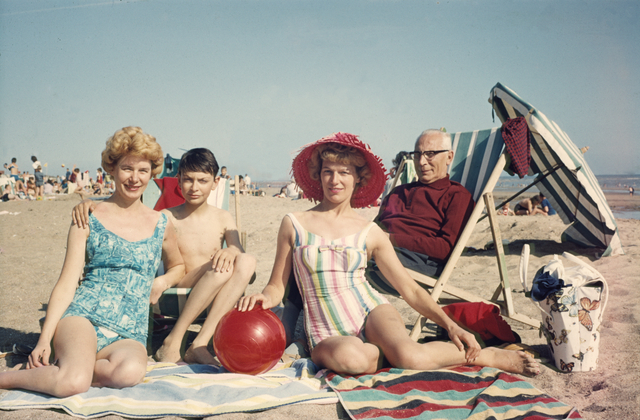
\includegraphics[width=0.495\textwidth]{DIA-0078-0352.jpg}\hfill
	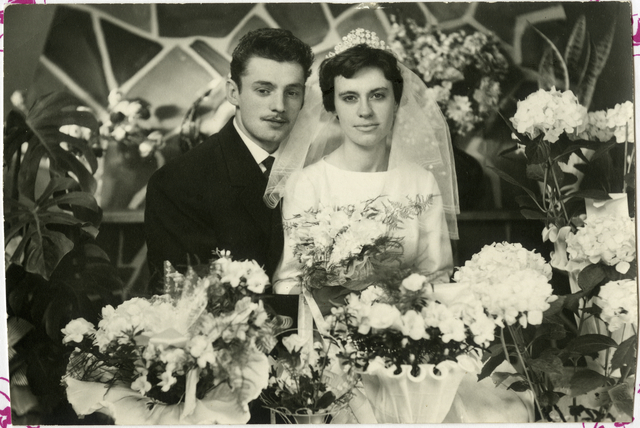
\includegraphics[width=0.495\textwidth]{FO-50-01658.jpg}\hfill
	\\[\smallskipamount]
	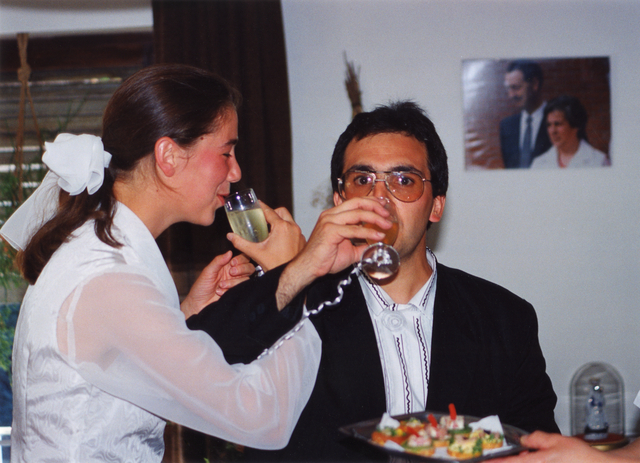
\includegraphics[width=0.57\textwidth]{FO-90-00157.jpg}\hfill
	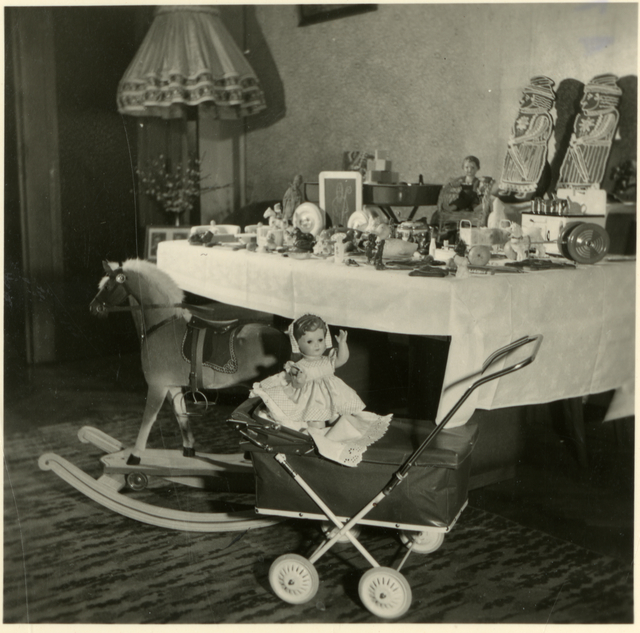
\includegraphics[width=0.42\textwidth]{FO-50-02073.jpg}\hfill
	\caption[Enkele voorbeelden van foto's die goed of slecht getagged werden door het ingbouwde Clarifai-model]{Drie foto’s uit de fotocollectie van Huis van Alijn waarvan alle tags correct waren en de foto waar het minst aantal tags correct waren (rechtsonder).}
\end{figure}

Vooraf hadden we verwacht dat het model niet goed zou scoren op de Sinterklaasfoto’s. Sinterklaas is immers een ritueel dat enkel voorkomt in de lage landen en enkele vroegere koloniën van Nederland. De kans lijkt dus klein dat het model de concepten van Sinterklaas kent. Omdat modellen voornamelijk getraind worden met hedendaagse foto’s, vreesden we ook dat de resultaten met de oudere foto’s minder goed zouden zijn.


Na validatie bleek het vermoeden rond de Sinterklaasfoto’s correct te zijn (zie tabel \ref{tab:analyse-resultaten-thema}). Het valt meteen op dat dit thema het laagste gemiddelde en het hoogst aantal foto’s met minder dan tien correcte tags heeft. Aan de beelden van dit thema werden tevens het minst aantal unieke termen gegeven. Het model blijkt ook minder goed op het speelgoedthema te scoren. De resultaten voor de huwelijksfoto’s zijn dan weer erg goed. Het gemiddelde voor dit thema is ongeveer 1,5 punten beter dan het gemiddelde van alle beelden.
	
\begin{table}
    \renewcommand\arraystretch{1.2}
    \centering
	\begin{tabular}{p{3cm}|ccccc}
	 	\toprule
		 & $\bar{x}$ (/20) & $\max$ & $\min$ & aantal unieke termen & aantal < 10 \\ 
		\midrule
		Geboorte & 13,69 & 20 & 7 & 112 & 7 \\ 
		Huwelijk & 15,16 & 20 & 8 & 158 & 7 \\ 
		Sint & 10,03 & 15 & 7 & 51 & 48 \\ 
		Speelgoed & 11,28 & 17 & 6 & 126 & 23 \\ 
		Vakantie & 13,42 & 20 & 9 & 212 & 12 \\ 
		Alle foto's & 13,63 & 20 & 6 & 371 & 97 \\ 
	\bottomrule
	\end{tabular} 
	\caption[een overzicht van de resultaten per thema na gebruikt van het ingebouwde model van Clarifai]{een overzicht van het gemiddelde ($\bar{x}$), maximale en minimale aantal juiste tags van de twintig tags van Clarifai voor de foto’s per thema, het aantal unieke termen dat gegeven werd aan ieder thema en het aantal foto’s waarvan minder dan tien tags correct waren. }
	\label{tab:analyse-resultaten-thema}
\end{table}

Wat betreft de periodes is het moeilijker om conclusies te trekken. Uit tabel \ref{tab:analyse-resultaten-periode} kan afgeleid worden dat de recentere foto’s (1960-1999) beter scoren en dat de oudste foto’s het slechtst scoren. Niettemin moet dit genuanceerd worden. Er zijn immers slechts negen beelden uit de jaren 1900. Bovendien bestaan foto’s uit de jaren 50 - en in mindere mate uit de jaren 40 - voor een groot deel uit foto’s over Sinterklaas, wat hun slechtere score kan verklaren. Foto’s uit de jaren 60 scoren opmerkelijk goed, maar dit valt dan weer te verklaren door de grote aanwezigheid van huwelijksfoto’s in die periode (meer dan 75\%).\footnote{zie \ref{sec:analyseren-van-de-dataset}}

\begin{table}
    \renewcommand\arraystretch{1.2}
    \centering
	\begin{tabular}{ll|cccccc}
		\toprule
		& &$\bar{x}$ (/20)&&  $\max$ && $\min$ &  aantal < 10 \\ 
		\midrule
		00s && 11,44 && 14 && 9 & 1 \\ 
		10s & &12,69 && 16 && 8 &  2 \\ 
		20s & &12,91 && 19 && 9 & 3 \\ 
		30s & &13,26 && 20 && 9 & 3 \\ 
		40s & &12,16 && 20 && 7 & 19 \\ 
		50s & &12,33 && 20 && 6 & 48 \\ 
		60s & &15,01 && 20 && 7 & 7 \\ 
		70s & &14,56 && 20 && 7 & 4 \\ 
		80s & &14,26 && 20 && 7 & 3 \\ 
		90s & &14,48 && 20 && 9 & 1 \\ 
		Onbekend && 12,76 && 20 && 9  & 6 \\ 
        \midrule
		Alle foto's && 13,63 && 20 && 6  & 97 \\ 
		\bottomrule
	\end{tabular} 
	\caption[een overzicht van de resultaten per periode na gebruik van het ingebouwde model]{een overzicht van het gemiddelde ($\bar{x}$), maximale ($\max$) en minimale ($\min$) aantal juiste tags per periode en het aantal foto’s waarvan minder dan tien tags (of de helft) correct waren. }
	\label{tab:analyse-resultaten-periode}
\end{table}

\section{Gedetailleerde resultaten per thema}
\label{sec:gedetailleerde-resultaten-per-thema}

In dit deel wordt dieper ingegaan op de resultaten per thema. Voor ieder thema wordt de top 30 van meest voorkomende termen, het maximale, minimale en gemiddeld aantal correcte tags, het aantal beelden met minder dan tien juiste tags en het aantal unieke termen toegelicht. 

\subsection{Geboorte}

In totaal waren er 96 beelden voor dit thema. De API scoorde goed op deze foto’s, in lijn met het totale gemiddelde. Er werden 112 unieke termen gebruikt om de beelden te beschrijven. Gemiddeld waren 13,7 tags correct. Het maximale aantal correcte tags was twintig, het minste zeven. Slechts zeven beelden hadden minder dan tien correcte tags (7,2\%).
\begin{table}
	\centering
	\begin{tabular}{*{3}{l}}
		mensen (93) & zoon (48) & gezichtsexpressie (22) \\
		volwassene (83) & 	groep (35) & meisje (19) \\
		kind (82) & twee (32) & affectie (17) \\
		vrouw (76) & sepia (29) & drie (16) \\
		portret (75) & binnenshuis (27) & verschillende (15) \\
		familie (65) & 	kamer (27) & broer of zus (13) \\
		kledij (62) & 	meubels (25) & bed (10) \\
		nageslacht (51) & liefde (25) & jongen (8) \\
		man (49) & samenkomen (24) & voertuig (7) \\
		baby (48) & monochroom (23) & stoel (7) \\	
	\end{tabular}
	\caption{De dertig meest voorkomende tags van geboortefoto's met het ingebouwde Clarifai-model}
	\label{tab:30-termen-geboorte}
\end{table}

\begin{figure}
	\centering
	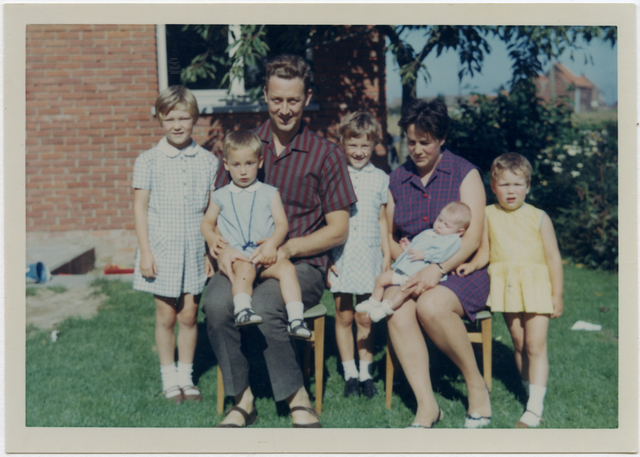
\includegraphics[width=\textwidth]{FO-60-01055.jpg}\hfill
    \\[\smallskipamount]
	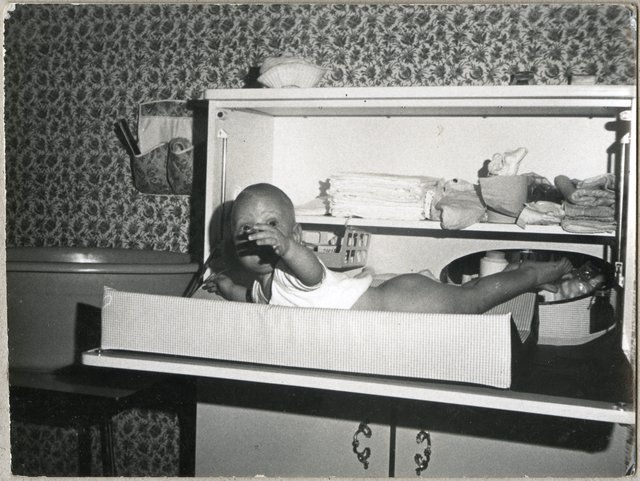
\includegraphics[width=\textwidth]{FO-70-00900.jpg}\hfill
	\caption[Best en slechtst scorende foto van thema geboorte]{een best scorende (boven) en slechtst scorende (onder) foto van het thema geboorte uit de fotocollectie van het Huis van Alijn.}
\end{figure}

De dertig meest voorkomende termen verwijzen naar mensen, kinderen en nakomelingen. Het model ziet ook enkele emoties in de beelden: liefde en affectie. Het merendeel van de foto’s waren ook portretten van moeder (en soms ook vader) met baby. Soms stonden er ook andere mensen, zoals broers, zussen, familieleden en vrienden op de foto. 

Uit de top 30 valt op dat er een groot verschil is tussen het aantal verschijningen van de meest voorkomende term (93 keer) en die op plaats 30 (7 keer). De top 11 komt in minstens de helft van de beelden voor. Het valt hierbij ook op dat term baby slechts aan de helft van de foto’s gegeven is.

Een opvallende vaststelling was dat het model de term \textit{dochter} niet kent; enkel \textit{zoon} werd gegeven. Doordat het voor ons niet mogelijk was om het verschil tussen een mannelijke en een vrouwelijke baby te zien, hebben we dit altijd als correct beschouwd.

Het model vergiste zich soms ook. Man en vrouw met kind werden in zestien van de gevallen door het model als een trouwfoto beschouwd. Ook de tags bruidegom (3 keer) en bruid kwamen voor (2 keer). Dit is vermoedelijk doordat op die foto’s de baby gewikkeld was in een sluier, wat verkeerdelijk door het model als een bruidssluier gepercipieerd werd.

\subsection{Huwelijk}
Voor dit thema waren vierhonderd beelden beschikbaar. Het general model van Clarifai scoorde erg goed op dit thema. Er werden 158 unieke termen gebruikt om de beelden te beschrijven. Gemiddeld waren 15,2 tags correct, wat ruim boven het gemiddelde is van alle beelden. Het maximale aantal correcte tags was twintig, het minste acht. Slechts zeven beelden hadden minder dan tien correcte tags, wat maar 1,75\% van het totaal aantal trouwfoto’s is!

\begin{figure}
	\centering
	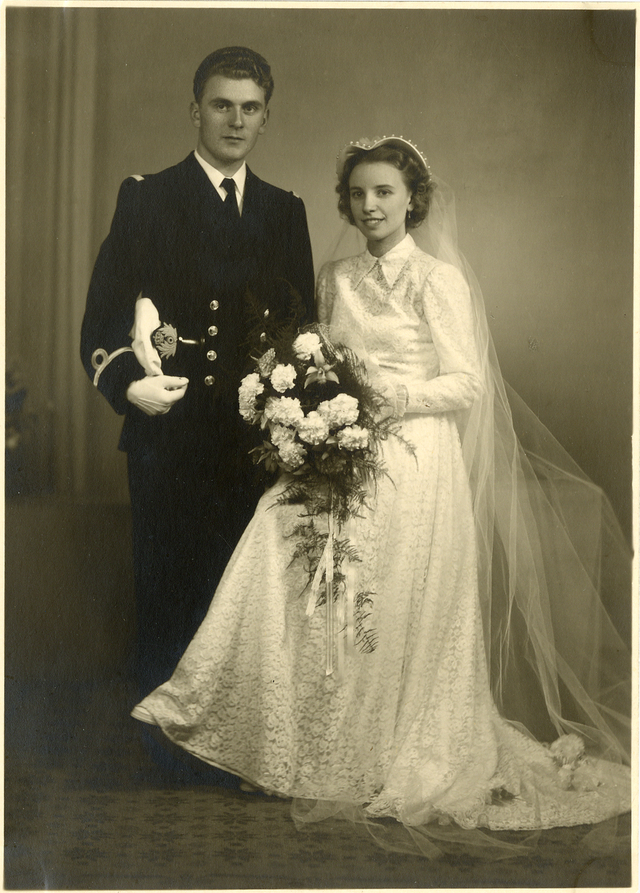
\includegraphics[width=0.505\textwidth]{FO-40-00650.jpg}\hfill
	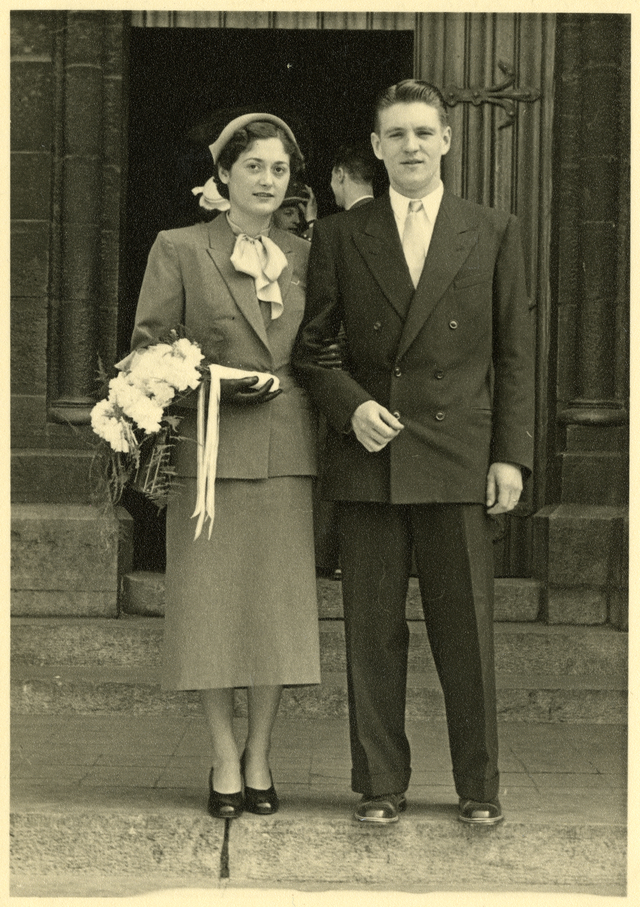
\includegraphics[width=0.495\textwidth]{FO-50-01313.jpg}\hfill
	\caption[Best en slechtst scorende foto van thema huwelijk]{een best scorende (links) en slechtst scorende (rechts) foto van het thema huwelijk uit de fotocollectie van het Huis van Alijn.}
\end{figure}

De dertig meest voorkomende termen verwijzen naar termen die je verwacht bij trouwfoto’s: mensen, een koppel, vrouw, man, bruid, bruidegom, boeket, op een bruiloft, in smoking en (trouw)jurk. Ook in deze foto’s wordt liefde gezien. 

De top tien van de termen komt in minstens de helft van de beelden voor. We stellen hier tevens een verschil vast tussen de meest (399 keer) en minst (48 keer) voorkomende term. Het valt op dat de term bruiloft 341 keer voorkomt; die van huwelijk 72 keer.

\begin{table}
	\centering
	\begin{tabular}{*{3}{l}}
		mensen (399) & sluier (198) & verschillende (83) \\
		vrouw (387) & groep (160) & smoking (75) \\
		volwassene (377) & jurk (159) & huwelijk (72) \\
		man (354) & ceremonie (147) & bruids (63) \\
		bruiloft (341) & gezichtsexpressie (132) & veel (58) \\
		portret (316) & samenkomen (127) & verbintenis (57) \\
		kledij (311) & liefde (121) & meisje (56) \\
		bruidegom (255) & monochroom (117) & koppel (55) \\
		twee (251) & bloemstuk (101) & kind (53) \\
		bruid (239) & familie (99) & boeket (48) \\	
	\end{tabular}
	\caption{De dertig meest voorkomende tags van trouwfoto's met het ingebouwde Clarifai-model}
	\label{tab:30-termen-huwelijk}
\end{table}

Uit analyse van de termen kan geconcludeerd worden dat het ingebouwde model van de Clarifai API trouwfoto’s kan onderscheiden zonder dat verdere training nodig is.

\subsection{Sinterklaas}

Zoals verwacht scoorde het Clarifai model niet goed op het taggen van de foto’s over Sinterklaas. Voor dit thema waren 97 beelden beschikbaar. Er werden slechts 51 unieke termen gebruikt om de beelden te beschrijven. Dit is 70 termen minder dan geboorte, dat na Sinterklaas de minst unieke termen heeft. Gemiddeld waren slechts tien tags correct, wat ruim onder het gemiddelde is van alle beelden (13,6). Het maximale aantal correcte tags was vijftien, het minste zeven. 48 beelden hadden minder dan tien correcte tags, wat 49,5\% van het totaal aantal Sinterklaasfoto’s is.

\begin{figure}
	\centering
	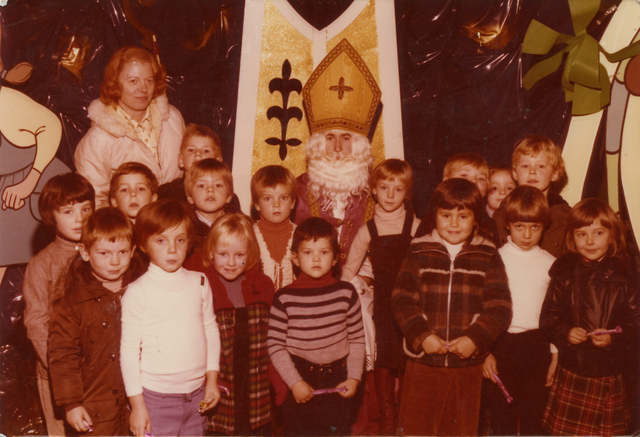
\includegraphics[width=0.67\textwidth]{FO-70-00254.jpg}\hfill
	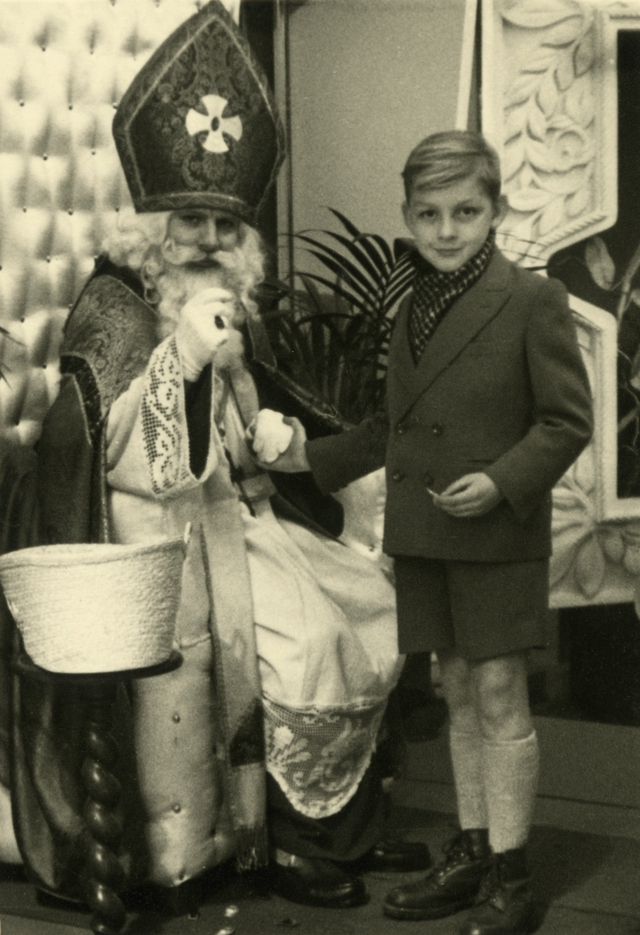
\includegraphics[width=0.32\textwidth]{FO-50-00439.jpg}\hfill
	\caption[Best en slechtst scorende foto van thema Sinterklaas]{een best scorende (links) en slechtst scorende (rechts) foto van het thema Sinterklaas uit de fotocollectie van het Huis van Alijn.}
\end{figure}

De reden voor deze lage cijfers komt zeer waarschijnlijk doordat het model de concepten van Sinterklaas niet kent. Het model gaf zeer regelmatig de tag \textit{retro} bij deze beelden, maar die werd steeds als incorrect aangevinkt. Alle beelden van Huis van Alijn zijn immers retro als het met hedendaagse ogen bekeken wordt. Daarnaast werden ook de termen \textit{zoon}, \textit{nakomelingen} en \textit{familie} als incorrect gevalideerd als er geen ouder of volwassene op de foto staat. 

De dertig meest voorkomende tags verwijzen naar een portret van twee, drie of vier mensen met volwassene(n) en kind(eren). De 97 beelden waren ook portretten van een of meerdere kinderen, soms vergezeld van volwassenen, met Sinterklaas. Wat opvalt is dat de tags sterk de nadruk op kleding leggen: kledij, sluier, outfit, kostuum, toga, bovenkleding. 

Ook bij deze beelden is er een groot verschil tussen de meest voorkomende termen en de minst voorkomende termen. Mensen en kledij komen in alle foto’s voor, terwijl meisje, toga en zitten voor slechts vijf foto’s gebruikt werden. De top 7 van de tags werd aan minstens de helft van de beelden gegeven. 

\begin{table}
	\centering
	\begin{tabular}{*{3}{l}}
		mensen (97) & drie (24) & broer of zus (10) \\
		kledij (97) & gezichtsexpressie (21) & vier (8) \\
		volwassene (95) & samenkomen (20) & bovenkleding (7) \\
		portret (91) & groep (19) & recreatie (7) \\
		kind (90) & kostuum (15) & acteur (6) \\
		man (86) & verschillende (15) & sepia (6) \\
		twee (53) & jongen (14) & uniform (6) \\
		monochroom (30) & vrouw (14) & meisje (5) \\
		outfit (30) & familie (13) & toga (5) \\
		sluier (25) & jas (10) & zitten (5) \\
	\end{tabular}
	\caption{De dertig meest voorkomende tags van Sinterklaasfoto's met het ingebouwde Clarifai-model}
	\label{tab:30-termen-sint}
\end{table}

\subsection{Speelgoed}

Er waren 101 foto’s voor dit thema. Net als bij Sinterklaas presteert Clarifai voor deze foto’s onder het gemiddelde. Gemiddeld waren 11,3 tags correct en hadden 23 beelden minder dan tien correcte tags (22,8\%). De slechts scorende foto had 6 juiste tags; voor de best scorende foto’s waren dit 17 tags. Voor het beschrijven van deze foto’s werden 126 unieke termen gebruikt.

\begin{figure}
	\centering
	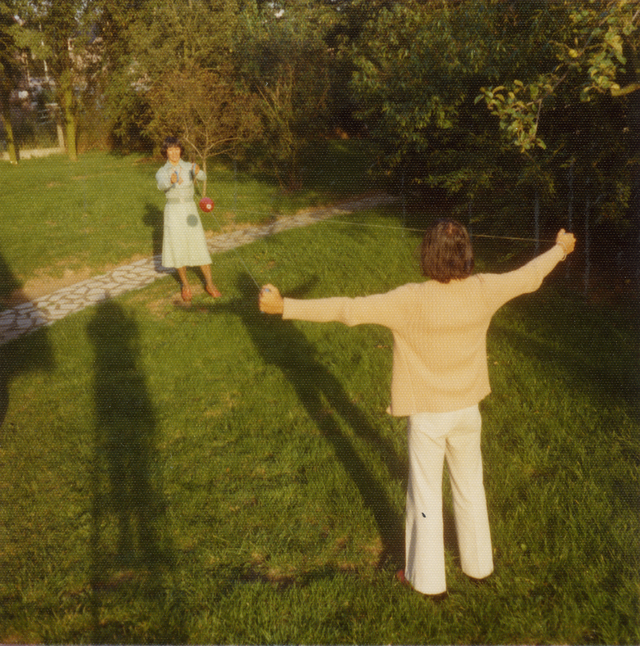
\includegraphics[width=0.495\textwidth]{FO-70-00621.jpg}\hfill
	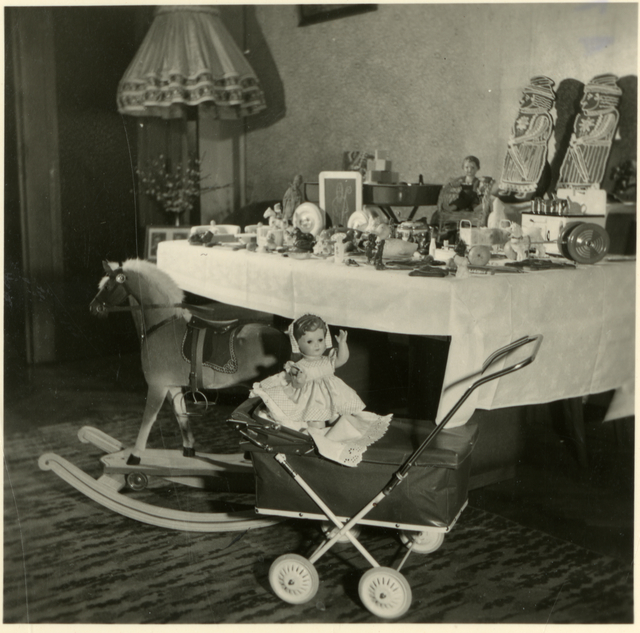
\includegraphics[width=0.495\textwidth]{FO-50-02073.jpg}\hfill
	\caption[Best en slechtst scorende foto van thema speelgoed]{een best scorende (links) en slechtst scorende (rechts) foto van het thema speelgoed uit de fotocollectie van het Huis van Alijn.}
\end{figure}

De dertig meest voorkomende termen verwijzen vooral naar kinderen, slechts in mindere mate naar speelgoed zelf. Het valt bijvoorbeeld op dat het afgebeelde speelgoed vaak niet herkend (of getagd) werd. Wel wordt er plezier en recreatie herkend. De term speelgoed (18 keer) komt ook voor, maar wel in mindere mate, net als vrije tijd (5 keer), spelen (5 keer) en spel (4 keer). Het ingebouwde model is bijgevolg niet voldoende om het merendeel van de speelgoedfoto’s eruit te halen.

De grote verschillen tussen de meest (100 keer) en minst (9 keer) voorkomende termen vallen op. Enkel de top 4 van de termen wordt aan minstens de helft van de beelden gegeven. Dit komt vermoedelijk omdat deze foto’s een minder vast format hadden dan de foto’s van de vorige thema’s. Die foto’s waren vaak portretten van resp. moeders/ouders met hun pasgeboren kind, bruid en bruidegom op hun trouwdag en kinderen met Sinterklaas. De speelgoedfoto’s hadden een grotere variëteit aan composities: portretten van kinderen die met hun speelgoed poseerden, maar ook kinderen en/of volwassenen die gezamenlijk een spel speelden. 

\begin{table}
	\centering
	\begin{tabular}{*{3}{l}}
		mensen (100) & recreatie (29) & speelgoed (18) \\
		kind (96) & twee (29) & broer of zus (17) \\
		kledij (65) & binnenshuis (28) & straat (17) \\
		portret (51) & familie (25) & voertuig (17) \\
		kamer (48) & groep (25) & thuis (16) \\
		jongen (44) & volwassene (22) & vrouw (14) \\
		monochroom (43) & zitten (22) & sepia (12) \\
		meisje (42) & samenkomen (20) & zitplaats (11) \\
		meubels (38) & gezichtsexpressie (18) & stoel (10) \\
		één (34) & plezier (18) & man (9) \\
	\end{tabular}
	\caption{De dertig meest voorkomende tags van de speelgoedfoto's met het ingebouwde Clarifai-model}
	\label{tab:30-termen-speelgoed}
\end{table}

Naar de reden voor de mindere score voor deze beelden is het gissen. Net zoals bij Sinterklaas werden vaak de termen \textit{retro} of \textit{vintage} gegeven, wat als fout beschouwd werd. Idem voor de termen \textit{zoon}, \textit{nakomelingen} of \textit{familie}, wanneer er geen ouder op de foto staat. Ook vergiste het model zich regelmatig. Kinderen werden vaak als volwassene getagd of kregen een fout gender (bv. een jongen die als meisje gezien werd). Poppen werden dan weer vaak als baby gelabeld. Het valt op dat de tags zich hoofdzakelijk op mensen concentreren. Mogelijk is het model minder goed in objectherkenning, maar dit moet verder onderzocht worden.

\subsection{Vakantie}

Het ingebouwde model van Clarifai scoorde goed op de 151 vakantiefoto’s, in lijn met het algemene gemiddelde.  Er werden 212 unieke termen gebruikt om de beelden te beschrijven. Gemiddeld waren 13,4 tags correct. Het maximale aantal correcte tags was twintig, het minste negen. Slechts twaalf beelden hadden minder dan tien correcte tags (8\%).

\begin{figure}
	\centering
	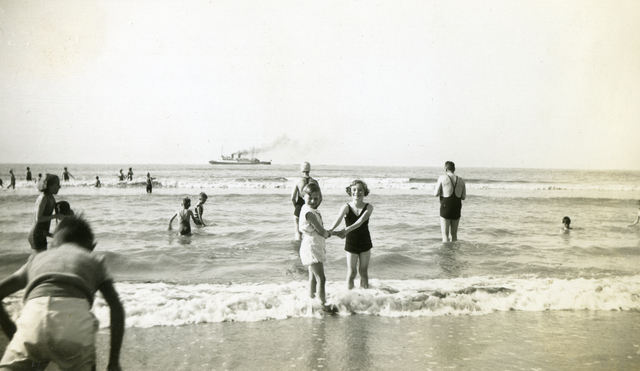
\includegraphics[width=\textwidth]{FO-30-00319_a3.jpg}\hfill
	\\[\smallskipamount]
	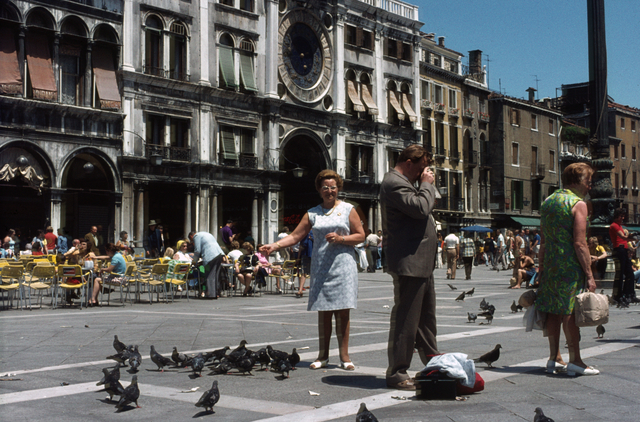
\includegraphics[width=\textwidth]{DIA-0006-0135.jpg}\hfill
	\caption[Best en slechtst scorende foto van thema vakantie]{een best scorende (boven) en slechtst scorende (onder) foto van het thema vakantie uit de fotocollectie van het Huis van Alijn.}
\end{figure}

De dertig meest voorkomende termen verwijzen naar mensen, vrije tijd, onderweg zijn en het strand. Het model ziet ook plezier in de beelden. Eveneens wordt het thema vakantie in negentien foto’s herkend, net zoals toerist (13 keer) en toerisme (8 keer).

Ook deze foto’s hebben geen vast format. Het zijn vakantiekiekjes. Dit verklaart de grote verscheidenheid aan termen om de beelden te beschrijven. De top 7 van de termen komt in minstens de helft van de beelden voor. Zoals bij de andere thema’s is er een groot verschil tussen het aantal verschijningen van de meest voorkomende term (142 keer) en de minst voorkomende term (17 keer). 

\begin{table}
	\centering
	\begin{tabular}{*{3}{l}}
		mensen (142) & straat (47) & meisje (23) \\
		volwassene (115) & voertuig (46) & weg (23) \\
		vrouw (98) & portret (35) & landschap (21) \\
		man (83) & veel (32) & water (21) \\
		recreatie (81) & strand (30) & vrije tijd (20) \\
		reizen (79) & monochroom (30) & vakantie (19) \\
		kledij (77) & buitenshuis (30) & familie (18) \\
		groep (75) & verschillende (30) & plezier (18) \\
		kind (50) & stad (26) & kust (18) \\
		samenkomen (48) & twee (25) & gebouw (17) \\
	\end{tabular}
	\caption{De dertig meest voorkomende tags van de vakantiefoto's met het ingebouwde Clarifai-model}
	\label{tab:30-termen-vakantie}
\end{table}

\section{Vergelijking met de beschrijvingen van registratoren}

De tags werden vergeleken met de beschrijvingen van de foto's door de menselijke registratoren. Hiervoor hadden we een export uit het collectiebeheersysteem van het museum gekregen van de 496 foto's van de thema's Sinterklaas en Huwelijk. 

Beschrijvingen bestonden uit:
\begin{itemize}
	\item Titel: de titel bestond meestal uit het afgebeelde onderwerp en personen, de locatie en de datum, bv. \textit{Huwelijk Juliette en Werner, Gent, 1962} of \textit{Meisje bij Sinterklaas, Grand Bazar Gent, 1949}.
	\item Beschrijving: geeft wat extra informatie over wat op de foto geportretteerd wordt.  Meestal wordt er meer informatie gegeven over de locatie op de foto, zoals \textit{Feestvierders komen aan in feestzaal de Raadskelder in Gent} of \textit{De foto werd genomen in de Grand Bazar in de Gentse Veldstraat}, maar soms wordt er ook meer duiding gegeven over de kledij of de personen op de foto.
	\item Objectnaam: Dit is steeds \textit{foto} of \textit{dia} voor de beelden in deze case.
	\item Creatiedatum van het object, steeds in de vorm jaar-maand-dag.
	\item Periode: het decennium waarin de foto genomen werd.
	\item Afgebeelde onderwerp: dit zijn termen die beschrijven wat op de foto afgebeeld is zoals \textit{huwelijk} of \textit{Sinterklaas}.
	\item Trefwoord: deze trefwoorden worden gebruikt om de collectie te doorzoeken. 
\end{itemize}

Het valt op dat er voor de verschillende beelden slechts een beperkt aantal velden ingevuld werden. Alle beelden hebben een titel, objectnaam en minstens een trefwoord (zie figuur \ref{fig:bestaande-beschrijvingen}). De andere velden werden minder ingevuld. Het veld \textit{beschrijving} werd zelfs maar voor 88 beelden ingevuld. Gebrek aan tijd en personeel zijn hier de oorzaak van, zoals reeds aangegeven in sectie \ref{sec:probleemstelling}. Huis Van Alijn pakt de registratie projectmatig aan. Wanneer er een tentoonstelling plaatsvindt, wordt de registratie van items over dat onderwerp aangepakt. Het museum heeft daarom thema's waarvan de beelden heel precies beschreven zijn, maar ook thema's waarbij dit minder het geval is. 

\begin{figure}
	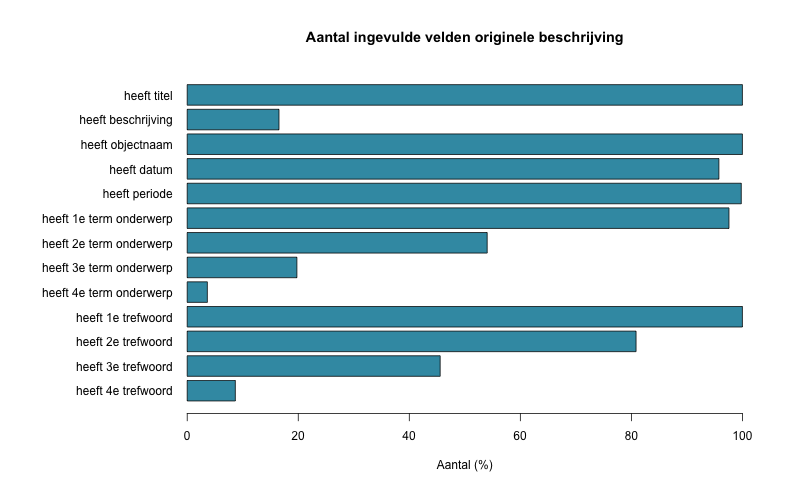
\includegraphics[width=\textwidth]
	{barplot_originele_beschrijvingen.png}
	\caption[Het aantal ingevulde velden in de bestaande beschrijvingen gemaakt door de registratoren van Huis van Alijn]{Een staafdiagram die aanduidt hoeveel velden (percentage) ingevuld werden door de registratoren van huis van Alijn. Het gaat enkel om de foto's van de thema's Sinterklaas en Huwelijk.}
	\label{fig:bestaande-beschrijvingen}
\end{figure}

Titel, beschrijving, periode en datum kunnen niet door Clarifai getagged worden, maar het is wel interessant om te kijken of het in staat is om afgebeeld onderwerp en trefwoord aan te duiden. De registratoren gebruikten 107 unieke termen voor deze velden. Dat is minder dan het aantal unieke termen dat door Clarifai gebruikt werd. Clarifai gaf gemiddeld minstens zes correcte tags aan ieder beeld (gemiddeld 13,6). Het valt uit figuur \ref{fig:bestaande-beschrijvingen} op dat de registratoren aanzienlijk minder termen geven aan de foto's: nog geen 50\% van de beelden heeft drie trefwoorden en ongeveer 50\% slechts twee afgebeelde onderwerpen. Vooral de Sinterklaasfoto's zijn erg beperkt beschreven. Bijna alle beelden van dit thema hebben slechts een trefwoord en afgebeeld onderwerp, namelijk de term \textit{Sinterklaas}. 

Elf van de de dertig meest voorkomende termen (zie tabel \ref{tab:30-termen-HvA}) zijn plaatsnamen. Dit zijn termen die Clarifai niet kan geven aan de beelden. Andere termen verwijzen vooral naar entiteiten die op het beeld te zien zijn (bruidspaar, park), informatie over de foto (studioportret en groepsfoto) en activiteiten (dans). Emoties of gevoelens, die Clarifai wel geeft, ontbreken. Het is opvallend dat een registrator slechts tien keer de term \textit{bruidegom} en zestien keer de term \textit{bruid} gebruikt heeft. Clarifai was in staat om die termen in dezelfde foto's respectievelijk 255 keer en 239 keer te herkennen.

De termen zijn doorgaans specifieker dan de termen van Clarifai (bruidspaar, bruidsboeket, huiskamer (zie tabel \ref{tab:30-termen-huwelijk})), maar het lijkt niet onmogelijk om op basis van de Clarfai-tags deze termen te verkrijgen. Clarifai geeft namelijk wel de termen \textit{huwelijk} en \textit{bloemstuk} of \textit{bloemen} waarvan de term \textit{bruidsboeket} afgeleid kan worden of de termen \textit{bruid} en \textit{bruidegom} waarvan de term \textit{bruidspaar} gemaakt kan worden.

\begin{table}
	\centering
	\begin{tabular}{*{3}{l}}
		huwelijk (400) & vervoer (34) & Merelbeke (12) \\
		bruidspaar (351) & dans (32) & Zomergem (12) \\
		Sinterklaas (192) & interieur (28) & Gentbrugge (11) \\
		bruidsboeket (189) & park (20) & behang (11) \\
		Gent (165) & huiskamer (17) & bruidegom (10) \\
		feest (94) & bruid (16) & Sint-Amandsberg (9) \\
		studioportret (57) & Sint-Martens-Latem (15) & taart (9) \\
		kerk (54) & Zwijnaarde (15) & Aalst (8) \\
		auto (36) & groepsportret (15) & Beervelde (8) \\
		bloem (plant) (34) & Veldstraat (Gent) (14) & Loppem (8) \\
	\end{tabular}
	\caption[De dertig meest voorkomende termen gebruikt door registratoren van Huis van Alijn]{De dertig meest voorkomende termen gebruikt door registratoren van Huis van Alijn voor Sinterklaas- en huwelijksfoto's. De term \textit{Sinterklaas} komt 192 keer voor omdat het als afgebeeld concept en trefwoord gebruikt werd.}
	\label{tab:30-termen-HvA}
\end{table}

Uit deze analyse concluderen we dat een ingebouwd model van een CV API in staat is om een registrator te ondersteunen bij het werk. Clarifai is sneller en vollediger en kan zo de foto's voorzien van meer termen. De meerwaarde van een CV API zit vooral in het aanbieden van een andere soorten inhoudelijke ontsluiting dan traditioneel door registratoren wordt voorzien. We hebben het dan over de tags die emoties aanduiden (liefde, plezier), maar ook conceptuele concepten (vrienschap, het samen zijn). Die termen zien we immers niet terugkomen bij de beschrijvingen van de registratoren. Die inhoudelijke termen geven de gebruiker de mogelijkheid om op andere manieren doorheen de collectiebeelden te struinen. Het dient verder onderzocht te worden of de service gebruikt kan worden om termen te genereren uit de termenlijst van Huis van Alijn. 

\section{Toepassen in de praktijk?}
\label{sec:ingebouwd-toepassen-praktijk}

Het loslaten van het ingebouwde model van Clarifai op de 845 beelden van Huis van Alijn leverde 11.517 juiste (68\%) en 5.383 foute (32\%) tags op. Dit gebeurde in ongeveer 35 minuten. Om dit in een productieomgeving te gebruiken, zijn een aantal strategieën mogelijk om het aantal fouten te verkleinen.

\subsection{Instellen van een drempelwaarde}

Er kan een drempelwaarde ingesteld worden om het aantal foute tags te verkleinen. Bij het instellen van een drempelwaarde worden alleen maar tags aanvaard waarvan de waarschijnlijkheidsscore groter is dan de drempelwaarde. Bij het uitvoeren van de case werd geen drempelwaarde ingesteld. De hoogste waarschijnlijkheidsscore van een correcte tag was 100\%, de laagste 64,7\%.

\begin{figure}
	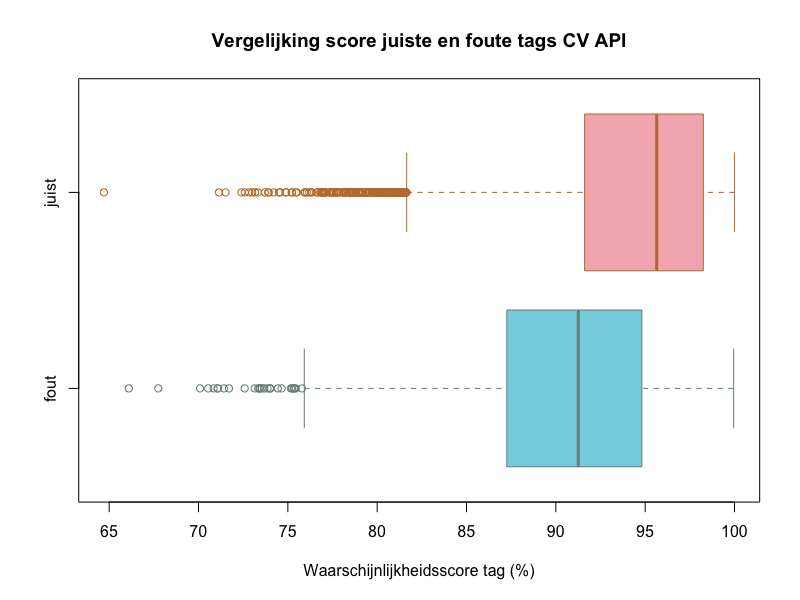
\includegraphics[width=\textwidth]
	{boxplot_tags_clarifai.png}
	\caption[Vergelijking van waarschijnlijkheidsscores juiste en foute tags]{Twee boxplots die de waarschijnlijkheidsscores vergelijken van tags van Clarifai die als juist en fout beoordeeld worden. Er is een overlap merkbaar tussen beide boxplots waardoor het niet mogelijk is om het grootste deel van de juiste tags te behouden en de fouten te vermijden bij het instellen van een drempelwaarde.}
	\label{fig:boxplot-clarifai}
\end{figure}

Indien het museum de drempelwaarde instelt op 90\%, krijgt het 82\% van het totaal aantal juiste tags. 25\% van de verkregen tags zijn dan fout. De drempelwaarde kan nog hoger gesteld worden, op 95\%, maar dan krijgt het slechts 55\% van het totaal aantal juiste tags. Slechts 17\% van de verkregen tags zijn dan verkeerd. De drempelwaarde kan verlaagd worden naar 85\% om een groter aandeel van de juiste tags te hebben, maar dan zijn 30\% van het aantal tags fout. Nu is dit aantal 32\% zonder drempelwaarde (tabel \ref{tab:instellen-drempelwaarde}).

\begin{table}
    \renewcommand\arraystretch{1.2}
    \centering
	\begin{tabular}{*{3}{c}}
		\toprule
		drempelwaarde (\%) & aandeel juiste tags (\%) & aantal foute tags (\%) \\
        \midrule
		95 & 55 & 17 \\
        [\smallskipamount]
		90 & 85 & 25 \\
        [\smallskipamount]
		85 & 95 & 306 \\
        [\smallskipamount]
		geen & 100 & 32 \\
		\bottomrule
	\end{tabular}
	\caption{Verhouding tussen drempelwaarde, totaal aantal van de juiste tags en het aantal foute tags}
	\label{tab:instellen-drempelwaarde}
\end{table}

\subsection{Selectie maken van thema’s}

Een andere strategie om fouten te verkleinen is om een selectie te maken van de foto’s die door de CV API gelabeld moeten worden. Het museum zou ervoor kunnen kiezen om thema’s waarmee het ingebouwde model niet vertrouwd is, niet te laten labelen, zoals bijvoorbeeld de Sinterklaasfoto’s. Deze foto’s doen immers het gemiddelde dalen en het aantal foute tags stijgen. Een nadeel aan deze strategie is dat de foto’s al op voorhand ingedeeld moeten zijn in thema’s.